\section{Discussion}\label{sec:discussion}

In this section we discuss about the %generalizability of the proposed solution (Section~\ref{sec:generalizability}), %. %the fault injection model is discussed. 
%Furthermore, 
%the 
lessons learned (Section~\ref{sec:lessonslearned}), the quality of findings and what benefits could be gained from the study (Section~\ref{sec:qualityOfFindings}), and the 
challenges of adopting the fault injection approach (Section~\ref{sec:challenges}). %are outlined. The section continues by discussing 
%and . %Finally future work and some keys of improvements are suggested.

\subsection{Lessons learned}\label{sec:lessonslearned}

\noindent {\bf Randomized testing}: Randomized testing is a cost-effective way to complement traditional testing, remove potential  developer bias, and identify unknown failure modes. This study indicated that fault injection can be feasible and applicable for testing the robustness and the dependability of the embedded distributed system. %As a result of this work we have discovered that fault injection techniques can be adapted to the embedded distributed components. 
%detected unexpected faults within distributed embedded systems

\noindent {\bf Randomization challenges}: First of all faults need to be more of the character of nuisances that the system should be able handle, such as (i) delays, (ii) lost messages, (iii) invalid data, and (iv) restarted instances. Then, we had the need of automatic use case validation to ensure the detection of errors introduced by the nuisances. However, the use case automation has to be relaxed to allow recovered errors to be ignored.
Reproduce-ability of errors is not simple since nuisances are random. Possible solutions are to use known seeds or to record and playback of events. Moreover, good traces are needed for post-mortem analysis of a crash. 

\noindent {\bf Producing good nuisances}: For what concerns the production of good nuisances, we had good results with (i) randomized delays, (ii) spurious signals, and (iii) randomized termination of instances. 

\noindent {\bf Context specific approach}: The fault injection strategy depends on the context although recurring patterns might be probably identified.  In particular, when considering embedded systems, it is necessary to interact with domain experts to understand which kind of faults should be injected, and also personalize the implementation of specific faults.

\noindent {\bf Adoption goes beyond technicalities}: Adoption in practice goes beyond technicalities, thus involving also organization, processes, and specificities of companies. Therefore, it is important to have a strong and continuous collaboration between academia and industry. Iterative development methodologies are a good strategy to enable continuous validation and collection of feedbacks from practitioners. %This reduces the risk of producing wrong solution. 



\subsection{Quality of findings}\label{sec:qualityOfFindings}

%The PM framework tested using the traditional testing methods such as unit and functional testing. 
%In traditional testing, test cases might not cover all the needed cases on how the system should perform. Therefore, the results will mainly depend on how well the test cases are written and how well do they cover what should be covered. For this reason, traditional testing can lack of detecting the unexpected faults. Utilizing the fault injection approach for testing the PM framework at the RBS will complement the traditional testing and add some value, since the fault injection approach is used to detect the dependability issues as well as the unexpected faults based on a random manner. Moreover, as described in \cite{testselectionnondeterministic} deterministic testing usually covers smaller test suites with full fault coverage, on the other side, non deterministic testing covers larger test suites. 

%As a result of running the fault injection tool, a
Even though the quality of system has been proven to be quite high, unexpected faults, which were not caught by traditional testing, were detected, such as: 

\begin{itemize}
\item fuzzing of signals has detected a weakness in handling dynamically sized objects causing a crash which then could be rectified, and 
\item randomized delays detected misconfigured timeout handling. It is important to highlight that the manual test case had the same mistake as the production code so this error was missed.
\end{itemize}

%Unfortunately, due to non disclosure agreements we cannot provide further details about the detected faults. 
The faults were identified and diagnosed by observing the stack trace on the log files. Diagnosing the faults helped us also in identifying the bottleneck of the distributed system. This has been shown after injecting the message delay fault type on the weak spots of the architecture that have strong coupling. After identifying the weak points, any improvement in the architecture will be easier to do. Moreover, detecting and diagnosing the faults also helped in discovering more faults to inject. 
%Detecting the unexpected faults and discovering the bottleneck of the software architecture at this stage will save money and time. Since distributed systems at Ericsson grow exponentially over time, detecting faults as early as possible will be very beneficial. Moreover, the confidence level of testing and code quality is increased and most probably, even the % Consequently, 
%customer satisfaction will increase.  

%As conclusion, this study indicated that fault injection can be feasible and applicable for testing the robustness and the dependability of the embedded distributed system. Furthermore, unexpected faults were detected using the fault injection approach. Moreover, this study can be taken as an inspiration on how to utilize fault injection techniques on embedded distributed systems in general.  



%\subsection{Generalizability}\label{sec:generalizability}
%
%The implementation of the fault injection tool was designed for RBS at Ericsson. 
%%Two fault types have been implemented and integrated to the automatic testing environment. The first fault type is sending random messages and the second one is delaying the messages.
%%
%%Fault injection techniques are widely used for testing the availability, robustness and the dependability of the software systems. Fault injection techniques are mainly used late on the development cycle after the software has been developed; there are some limitations when utilizing the fault injection in an early stage presented in \cite{rana2013improving}. To come over those limitations fault injection shall be combine with other testing like mutation testing for adapting it in an early stage of the development process \cite{rana2013improving}. 
%%The approach that has been developed in this thesis can be adapted late in the development cycle after the software has been implemented. Moreover, it 
%However, the approach presented in this paper is general and can be applied on distributes systems that consist of small embedded components.
%The constrains and requirements that should be considered when utilizing this approach in other context which are:    
%%\begin{itemize}
%%    \item T
%(i) the programming language should be C/C++ while the injections are performed on the top of the HW layer; 
%%    \item E
%(ii) embedded distributed environment; 
%%	\item L
%(iii) limited computation power of the small embedded components; 
%%	\item T
%(iv) the platform should be based on Linux or Unix; 
%%	\item T
%(v) there should be some shared libraries supporting existing functionalities such as send/receive signals; 
%%    \item T
%(vi) the system should follow the process and thread communication paradigm; and 
%%	\item Wrapping the sharing library. 
%%    \item T
%(vii) there must be some existing test cases and/or test suites.  
%%  \end{itemize}
%
%%Figure~\ref{Fualt_injection_Model} shows some general components that should be included in order to adapt this approach.
%
%As a result of this work we have discovered that fault injection techniques can be adapted to the embedded distributed components. 

%\subsection{Fault injection model}

%Figure \ref{Fualt_injection_Model} presents the fault injection model, which consists of the target system (PM\_fwk), fault injector, monitor (log files), IPC library as well as the controller that has the automatic testing and the configuration files.
%
%After running the fault injection tool all data are monitored from the log files using stack trace, these data are collected and analyzed for the evaluation of the tool as well as for answering the main research questions. The user can run and control the tool through the controller, where the automatic testing environments and the configuration files are located. Through the automatic testing environment different testing techniques are listed. The fault injection tool supports random mechanism where the number of faulty messages, message delay and the time interval between sending the messages are randomized based on reasonable manner. On the other hand, the user can manually adjust the test cases through the configuration files.    
%
%
%The fault injection approach provides different fault types at different location and time. We have developed two fault types the first fault type is sending random messages and the second one is delaying the messages. Fault types such as sending invalid messages and delaying the messages were done by linking some dynamic libraries of IPC during run time. IPC library is a separate component, which consist of different system functionalities such as sending the messages between different system component. After deep study of the PM framework documentation and discussion with the supervisor, system targets were identified. The system targets were some critical components of the PM framework where they have strong dependencies. The faults were injected on the system target where there is strong coupling. Due to the fact that time factor can have an effect on running the experiments and to make sure that the result we got are reliable, we have repeated the experiments more than once at different time. For non deterministic testing as pointed in \cite{testselectionnondeterministic}, as long as the number of the repetition of test sequence increases, the quality of testing will also be increased. In actual testing this number is limited due to economical and practical reasons. However, when executing the testing large number of time, the probability that not all possible execution paths are executed will be close or even equal to zero.  
%
%\begin{figure}[h]
%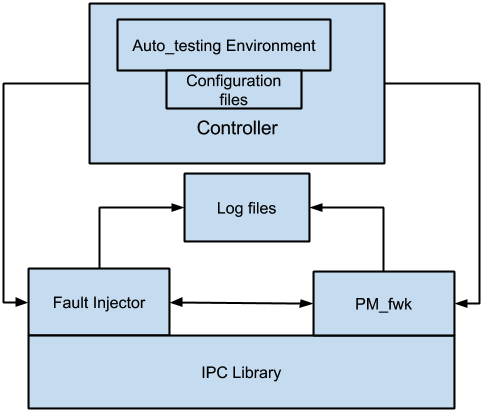
\includegraphics[width=\columnwidth]{figure/Fualt_injection_Model.png}
%\caption{Fault Injection Model \label{Fualt_injection_Model}}
%\end{figure}

\subsection{Challenges in adopting the fault injection approach}\label{sec:challenges}
During this study, we have met some challenges and barriers when adopting the fault injection approach. 
%Challenges started from understanding the existing system, since the software at the RBS in Ericsson is huge and complex as well as the number of the connected components are relatively high. 
%Furthermore, the idea of the fault injection is just available for cloud based application, but not to the embedded distributed system. So this study presents a new approach of fault injection that can be applicable to the embedded distributed system.  
%
%Another challenge was when we implemented the fault types, we implemented them from the scratch as well as imported some shared libraries in order to call some existing functionalities from the lower level. We met some difficulties in loading the IPC libraries as well as setting up the environment variables. After the implementation of the fault types, integrating the fault injection tool with the automatic testing environments was not a trivial task due to the strict conditions on the automatic testing environments. 
%
%There are some consideration that should be kept in mind when adopting this approach: 
%\begin{itemize}
%\item {\em Negative side effects}: When sending a lot of random messages without any time interval between the messages, 
% the system will probably crash since the computation power is limited on the embedded components. As stated in~\cite{Ali2014} online testing 
%could produce negative side effects out of the tester's control.
%It is then important to take into account also policies that help preventing or ameliorating such adverse
%effects. Also, as stated in~\cite{Ali2014}, online testing could have negative impact on nonfunctional characteristics; this can be mitigated by trading off
%testing accuracy with performance.
%%\item {\em Unrealistic results}: The testing method used in the fault injection approach is non-deterministic provocation thus the testing can catch unexpected faults that are seldom happened. When utilizing fault injection approach the results of the provoking can be both realistic and not realistic and this can be due to the fact that the input of the test is totally randomized. In order to mitigate from this limitation we made our test cases less randomized such as having time interval, specify the messages type, number of messages and delaying time. By doing this the result of the fault injection tool was more reasonable and at the same time it gave a realistic indicate when evaluating the system.
%\end{itemize} 

\noindent {\bf Unrealistic results}: Considering %Under the fact 
that %fault injection technique is 
we proposed a non-deterministic testing approach %that follow a randomized manner, 
the result of running such technique can be misleading. Doing a complete randomization of the test cases might produce useless results since the generating test case can be unrealistic. In order to mitigate this limitation we made our test cases less randomized such as having time interval, specify the messages type, number of messages and delaying time. 
For instance, when we implemented the first fault type, which was sending random messages, the system acts always differently. That was due to the fact that the injection is performed on embedded distributed systems with limited computation power. 
%where the computation power is limited, s
Sending a lot of random messages without any time between them was misleading. We come over this problem by inserting delays between each message sending. As a conclusion, having the time between each sending gave us a reasonable and realistic indication. 

\noindent {\bf Negative side effects}: When sending a lot of random messages without any time interval between them, 
 the system will probably crash since the computation power is limited on the embedded components. As stated in~\cite{Ali2014} online testing 
could produce negative side effects out of the tester's control.
It is then important to take into account also policies that help preventing or ameliorating such adverse
effects. Also, as stated in~\cite{Ali2014}, online testing could have negative impact on nonfunctional characteristics; this can be mitigated by trading off
testing accuracy with performance.

The strategy we adopted to avoid undesired crashes of the overall system because of injected fault is as follows:  
(i) Delaying signals - we make sure the delays fall within what the system should handle; (ii) Fuzzying signals - we limit fuzzying to faking Confirm/Rejects which the system should discard. %In the current state it is still hard for the PMFWK middleware to detect invalid Requests so that's left out.

%When we implemented the second fault type which was message delay, the system usually did not act as it should be, this was due to the fact that the time interval of delaying the messages was completely randomized. We come over this challenge by making it less randomized through identifying the default time and specifying the time interval. After that, the results were realistic and also gave us a reasonable indicate of approach evaluation. 
%Finally, continuous testing of the new implemented fault injection tool was time consuming. There are some steps that should be performed such as running the simulation and restarting the Erlang nodes in order to get and observe the result of testing in the log files. 



%Concluding, randomized fault injection can be an important test signal.

%\subsection{Altro}
%
%Online testing, however, poses two major challenges.
%First, it could produce negative side effects, out of the
%tester?s control, on the services of participating organizations.9
% The governance framework would thus need to
%include policies that help prevent or ameliorate such adverse
%effects, or compensate participating organizations
%in the event of serious consequences. Second, online testing
%could adversely impact nonfunctional characteristics.
%System engineers could mitigate this impact by trading off
%testing accuracy with performance.Preso da~\cite{Ali2014}



